
\chapter{INTRODUCTION}
\lipsum[1-4]~\cite{anderson1964hard}.

Test text Test text Test text Test text Test text Test text Test text Test text Test text Test text Test text Test text Test text 
Test text Test text Test text Test text Test text Test text Test text Test text Test text Test text Test text Test text Test text 
Test text Test text Test text Test text Test text Test text Test text Test text Test text Test text Test text Test text Test text 
Test text Test text Test text Test text Test text Test text Test text Test text Test text Test text Test text Test text Test text~\cite{khalil2012analysis}.

Test text Test text Test text Test text Test text Test text Test text Test text Test text Test text Test text Test text Test text 
Test text Test text Test text Test text Test text Test text Test text Test text Test text Test text Test text Test text Test text 
Test text Test text Test text Test text Test text Test text Test text Test text Test text Test text Test text Test text Test text 
Test text Test text Test text Test text Test text Test text Test text Test text Test text Test text Test text Test text Test text~\cite{sage2015study}.

\section{Intro:section I}
\lipsum[1-4]~\cite{anderson1964hard}

\begin{figure}[!t]
	{
	\begin{center}
		\begin{tabular}{c}
			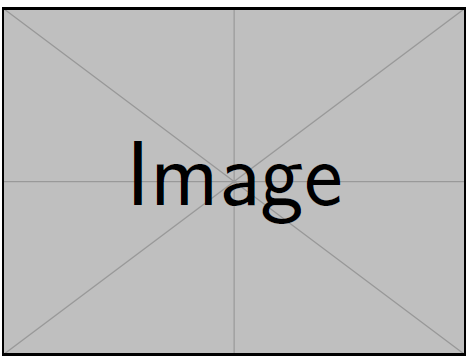
\includegraphics[width=0.9\linewidth]{dummy.png}
		\end{tabular}
	\end{center}
	}
	\caption[dummy image FIXME1]{Figure option of $!\text{t}$~\cite{chen2014fabrication}.}
\label{dummy_img1}
\end{figure}

\subsection{Intro:section I-1}
\lipsum[1-4]~\cite{anderson1964hard}.

\begin{figure}[!b]
	{
	\begin{center}
		\begin{tabular}{c}
			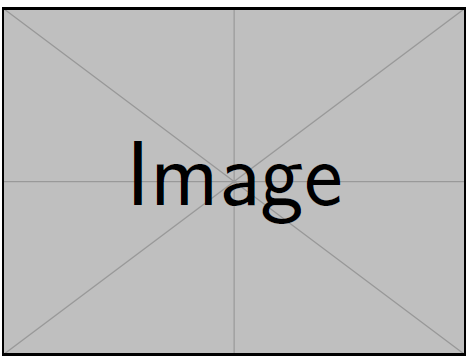
\includegraphics[width=0.9\linewidth]{dummy.png}
		\end{tabular}
	\end{center}
	}
	\caption[dummy image FIXME2 with long long long long long long long title]{Figure option of $!\text{b}$~\cite{Niepce2020geometric}.}
\label{dummy_img2}
\end{figure}

\section{Intro:section II}
\lipsum[1-4]~\cite{anderson1964hard}

\begin{table}[htbp]
	\renewcommand{\arraystretch}{1.6}
	\setlength{\tabcolsep}{10pt}
	\caption{Table caption goes up FIXME}
	\label{tbl2_1}
	\centering
	\begin{tabular}{l l l l l l c}
	\hline\hline
	Material & $T_c$ & $B_c$& $\xi$ & $\lambda_L$ & $\kappa$ & Type \\
	\hfill & [K] & [T] & [nm] & [nm] & \hfill & \hfill \\
	\hline
	FIXME & 1 & 2 & 3 & 4 & 5 & FIXME \\
	\hline\hline
	\end{tabular}
\end{table}

\subsection{Intro:section II-1}
\lipsum[1-4]~\cite{anderson1964hard}

\begin{sidewaystable}[htbp]
	\renewcommand{\arraystretch}{1.2}
	\setlength{\tabcolsep}{5pt}
	\centering
	\footnotesize
	\begin{tabular}{l c c c c c c c c c c c c c c c c c c c}
	\hline
	Parameter (FIXME) & P1 & P2 & P3 & P4 & P5 & P6 & P7 & P8 & P9 & P10\\
	\hline
	\multicolumn{11}{l}{\textbf{Conductor configuration}}\\
	$P_{FIXME}$\hfill[A]& FIXME & FIXME & FIXME & FIXME & FIXME & FIXME & FIXME & FIXME & FIXME & FIXME\\
	\hline
	\end{tabular}
	\caption{Key parameters of FIXME sideway table.}
	\label{tbl2-2}
\end{sidewaystable}